\chapter{Introduction}


%%%%%%%%%%%%%%%%%%%%%%%%%%%%%%%%%%%%%%%%%%%%%%%%%%%%%%%%%%%%%%%%%%%%%%%%%%%%%%%%%%%%%%%%%%%%%%%%%%%%%%%%%%%%%% 
% Présentation Contexte 
% Présenter le projet, le contexte. GUIMUTEIC, caméra, visite, action utilisateur.
% Aide à l'utilisateur : réagir à l'intention de l'utilisateur, approt d'information sur ce qui est regardé
\section{Le Contexte de cette thèse}

Les sites touristiques, et notamment les musées, ont su assimiler les évolutions technologiques et proposer de nouvelles méthodes d'interaction pour enrichire les visites et permettre des visites personnalisées.
La visite d'un site touristique peut être accompagnée d'un guide, ce dernier pouvant être humain, un guide culturel, ou électronique.
Ces nouveaux outils ne remplacent pas un guide humain, mais permettent de fournir des informations visuels, visio-guide, ou des informations audio, audio-guide.
Ces outils pouvant être mobile ou fixe, comme des bornes multimédia.
Grâce aux avancées techniques, telles que la réduction de la taille des capteurs ou la puissance des processeurs mobile, les possibilités d'outils mobilent s'enrichissent.

En examinant ces nouveaux usages et de leur impact~\cite{andr2014}, nous pouvons imaginer de nouvelle pratiques, avec des visites plus personnalisées.
Que ce soit réalité augmenté ou identification automatique du contexte dans lequel se trouve l'utilisateur, ces systèmes, reposent sur des procédés capables de reconnaître l'environnement qui entoure l'utilisateur.

Plus précisément, cette thèse s'inscrit dans le cadre d'un projet du Fonds unique interministériel (FUI) GUIMUTEIC. 
Ce projet a pour but de proposer une nouvelle génération de guides pour les visites de musée.
Equipé de différents capteurs, notamment une caméra, le dispositif GUIMUTEIC, équipant chaque utilisateur, est destiné à enrichir la visite, en la personalisant et en aidant à l'interaction.
Pour cela, le système GUIMUTEIC doit être capable d'identifier les points d'intérêts regardés par l'utilisateur, de le renseigner lorsque celui ci le désire, et de réagir en fonction des actions de ce dernier.
Ce travail de thèse explore en particulier les besoins d'identification d'oeuvres, d'actions et de l'environnement de l'utilisateur. 


\begin{figure}%
\centering
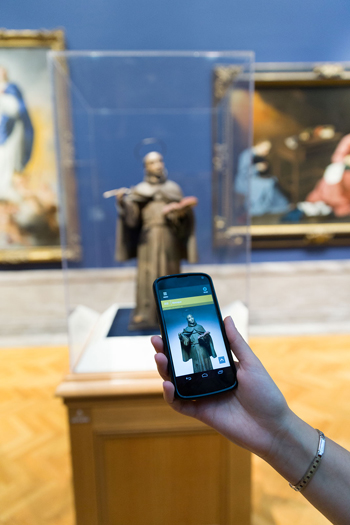
\includegraphics[width=\columnwidth/2]{figures/ArtLens.jpg}%
\caption{Exemple de visite avec une guide sur smartphone}%
\label{fig:exemplevisite}%
\end{figure}



%%%%%%%%%%%%%%%%%%%%%%%%%%%%%%%%%%%%%%%%%%%%%%%%%%%%%%%%%%%%%%%%%%%%%%%%%%%%%%%%%%%%%%%%%%%%%%%%%%%%%%%%%%%%%%
% PROBLEMATIQUE
% Reco d'oeuvre
% Reco d'action
% Reco de contexte
% Travail sur image et vidéo
\section{Problématiques et de recherche d'information muséale}
\label{sec:introcontraintes}
Les problématiques soulevée portent sur l'aide pouvant être apportée à l'utilisateur et les moyens d'interactions.
Équipé du dispositif GUIMUTEIC, donc d'une caméra embarqué, le but est de fournir à l'utilisateur une information sur son environnement, notamment les œuvres se trouvant face à lui.
Pour cela, il est nécessaire d'utiliser des méthodes d'indentification d'instances précises.
Nous référons ici par ``{\it Instance}'', l'instance d'un objet, par exemple la Jaconde, par opposition à une classe d'objet, dans ce cas un tableau. 

Une autre problématique est de déterminer si l'utilisateur souhaite avoir accès à une information. 
Nous avons besoin de détecter si, et à quel moment, l'utilisateur désir cette information.
En prenant comme exemple le musée de Bibracte~\footnote{\url{http://www.bibracte.fr/}}, ou certaines actions de déclenchent quand le visiteur entre dans une pièce, on voit l'intérêt de réagir en fonction des actions de l'utilisateur.
La localisation n'étant pas nécessairement suffisante~\cite{Locationisnotenough}, nous allons nous intéresser à des méthodes de détection des actions de l'utilisateur grâce au dispositif GUIMUTEIC.
 
 


%%%%%%%%%%%%%%%%%%%%%%%%%%%%%%%%%%%%%%%%%%%%%%%%%%%%%%%%%%%%%%%%%%%%%%%%%%%%%%%%%%%%%%%%%%%%%%%%%%%%%%%%%%%%%
% CONTRAINTES du projet
% Puissance limité
% Limitation sur les corpus
%\section{Contraintes du projet GUIMUTEIC}
%\label{sec:introcontraintes}
En dehors des problématiques scientifiques énoncées ci-dessus, nous avons signalé plus haut que ce travail s'inscrit dans le cadre du projet ``industriel'' GUIMUTEIC.
Ce cadre défini entre autre un certain nombre de contraintes qui vont influencer les choix effectués par la suite. 
Tout d'abord, cet outil est à destination de sites touristiques pouvant être de nature différentes, que ce soit en plein air ou dans un musées. 
De même, le type des oeuvres présent dans un musée est très variable, de pierres taillées dans un musée d'archéologie, à des peintures ou des oeuvres abstraites dans un musée moderne, en passant par des voitures ou des pièces de monnaies.
L'objectif est de fournir une solution général, pouvant s'adapter à chacun, avec un effort minimum.

Un autre contrainte directement lié au caractère industriel du projet, est l'effort de mise en place dans chacun des musées, qui doit être minimisé. 
L'acquisition des données, la quantité pouvant être recueilli ou l'annotation de ces données, sont des opérations coûteuses qui doivent être limitées. 
L'objectif étant de proposer une solution applicable aisément à chaque musée, le travail demandé pour la mise en place doit être aussi limité que possible.
L'étude de ces contraintes et de leurs impacts sur les choix pouvant être fait sera présenté dans le chapitre~\nameref{chap:etude}.




%%%%%%%%%%%%%%%%%%%%%%%%%%%%%%%%%%%%%%%%%%%%%%%%%%%%%%%%%%%%%%%%%%%%%%%%%%%%%%%%%%%%%%%%%%%%%%%%%%%%%%%%%%%%%
% OBJECTIFS et CONTRIBUTION
\section{Contributions}

Les objectifs de cette thèse sont multiples : nous nous intéresserons à la reconnaissance d'instance et explorer différentes méthodes d'interaction avec l'utilisateur, tout en respectant contraintes du projet GUIMUTEIC. 


%%%%%%%%%%%%%%%%%%%%%%%%%%%%%%%%%%%%%%%%%%%%%%%%%%%%%%%%%%%%%%%%%%%%%%%%%%%%%%%%%%%%%%%%%%%%%%%%%%%%%%%%%%%%%
% CONTRIBUTIONS
% La reco d'oeuvre
% La reco de geste
% Ouverture sur la reco de contexte
% La detection automatique de régions
% Detection d'intension de l'utilisateur : apprentissage des moments d'intérêt dans la vidéo. 
Ce travail de thèse apporte les contributions suivantes :
\begin{description}
	\item[Etude de l'accès à l'information pendant une visite touristiques] La première contribution de ce travail de thèse concerne l'étude des visites de musée et les besoin en terme d'accès à l'information pendant les visites touristiques. 
Nous étudions le développement de technologie dans le cadre de visites touristiques pour permettre une visite personnalisé avec de nouvelle méthode d'intéraction pour l'utilisateur, pour un accès à l'information en mobilité. 
	\item[Reconnaissance d'instance] Nous nous intéressons à l'identification d'instance, dans le but de reconnaître les scènes vues par l'utilisateur. Pour cela, nous étudierons l'apprentissage de similarité entre les images, à base de réseaux de neurones siamois.
	\item[Apprentissage des régions d'intérêt] Dans le but d'améliorer la reconnaissance d'instance, nous proposerons une nouvelle méthode d'apprentissage automatique des régions d'intérêt dans les images. Nous étudierons l'apport de cette détection sur l'apprentissage de similarité, et comment apprendre les deux conjointement.
	\item[Detection de geste] Pour proposer une interaction avec l'utilisateur, nous chercherons à détecter les gestes et actions de l'utilisateur grâce au dispositif GUIMUTEIC, c'est à dire avec une vue à la première personne (égocentrique). Nous allons pour cela nous intéresser à l'apprentissage de réseaux de neurones sur les vidéos.
	\item[Création de corpus d'évaluations] Pour vérifier la faisabilité du système développé dans des conditions réels, nous avons recueilli plusieurs corpus dans les musées partenaires du projet. Tous les algorithmes développés dans cette thèse seront évalués sur ces corpus. La collecte et l'organisation de ces corpus sera présenté en annexe~\ref{chap:corpus}.
\end{description}


%%%%%%%%%%%%%%%%%%%%%%%%%%%%%%%%%%%%%%%%%%%%%%%%%%%%%%%%%%%%%%%%%%%%%%%%%%%%%%%%%%%%%%%%%%%%%%%%%%%%%%%%%%%%%
% ORGANISATION de la thèse
\section{Plan du manuscrit}

Afin de mettre en place un système d'analyse d'information multimédia, nous allons réaliser une série de traitements, d'analyses et de méthodologies, que nous allons présenter dans ce manuscrit. 


\begin{description}
	\item[Chapitre~\ref{chap:etude}~\nameref{chap:etude}] Nous allons tout d'abord réaliser une étude approfondie du problème d'accès à l'information dans le cadre de visite touristiques. Nous analyserons plus en détail les contraintes spécifiques aux musées. Nous allons nous intéresser aux différents moyens d'accès à l'information développable dans ce contexte. 

	\item[Chapitre~\ref{chap:stateoftheart}~\nameref{chap:stateoftheart}] Ici, Nous allons présenter une introduction aux différentes méthodes de recherche d'informations multimédia et d'analyse d'image existantes dans la littérature. Nous présenterons l'état de l'art de la recherche d'image, ainsi que l'état de l'art de la détection d'évènements dans les vidéos. Nous allons également explorer différentes méthodes qui nous utiliserons par la suite pour developper nos propres solutions. Un état de l'art de méthodes d'évaluation de l'annotation de séquence sera aussi présenté.

	\item[\textbf{Chapitre~\ref{chap:similarite}~\nameref{chap:similarite}}] Dans ce chapitre nous allons présenter l'analyse et la modélisation du problème d'identification d'oeuvre dans les images et vidéos. Nous allons explorer différentes méthodes basées sur ce qui a été présenté dans le chapitre~\ref{chap:stateoftheart}. Nous présenterons également une nouvelle méthode pour la détection de régions d'intérêt dans les images. Nous évaluerons ces méthodes sur un corpus d'image créer spécialement.  

	\item[\textbf{Chapitre~\ref{chap:gestes}~\nameref{chap:gestes}}] Ce chapitre sera consacré à l'étude de la detection des actions de l'utilisateur dans les vidéos. 
	Suite à l'étude réalisée dans le chapitre~\ref{chap:etude}, nous nous intéresserons aux gestes nécessaire à l'interaction, et aux méthodes de détection pouvant être developpées. Nous étudierons comment détecter les gestes avec une vue à la première personne, à l'aide de réseaux de neurones sur les vidéos.

	\item[\textbf{Chapitre~\ref{chap:conclusion}~\nameref{chap:conclusion}}] Finalement, le dernier chapitre présente la démarche générale. Nous montrerons la mise en place du système sur le dispositif GUIMUTEIC. Nous conclurons sur les contributions de ce travail de thèse, et sur la suite des recherches possible sur les problématiques présentées.

\end{description}
